\subsection{Progettazione di Dettaglio e Codifica}
Dal 2020-03-16 al 2020-04-19\\
Inizia al termine della fase di Progettazione Architetturale e finisce con la data di consegna della Revisione di Qualifica.\\
In questa fase si definisce nel dettaglio e si implementa l'architettura logica costruita nella fase di Progettazione Architetturale.

\subsubsection{Periodo 1} 
Dal 2020-03-16 al 2020-03-27\\
\begin{itemize}
	\item \textbf{Approfondimento delle tecnologie}: Ricerca documentazione e materiali utili per l'apprendimento delle nuove tecnologie da utilizzare per la realizzazione del prodotto finale;
	\item \textbf{Normazione}: Standardizzazione e correzione di alcune parti della documentazione e che non aderiscono completamente alle \NdP{};
	\item \textbf{Correzioni}: Correzioni di difetti notati dal committente (ove presenti) nella \glo{Technology Baseline};
	\item \textbf{Assegnazione dei ruoli di progetto}: Assegnazione dei ruoli di ciascun membro del gruppo in base alla suddivisione oraria indicata in §5.3.1;
	\item \textbf{Pianificazione delle attività}: Le attività da svolgere devono essere prima pianificate e discusse dal gruppo per garantire il \glo{way of working} sancito nelle \NdP{};
	\item \textbf{Codifica}: Implementazione dei requisiti di base identificati per ottenere un sistema stabile;
	\item \textbf{Manuali}: Stesura del Manuale Utente e del Manuale Manutentore in relazione alle funzionalità di base del sistema.
\end{itemize}
\subsubsection{Periodo 2} 
Dal 2020-03-28 al 2020-04-08\\
\begin{itemize}
	\item \textbf{Progettazione di dettaglio}: A partire dalla progettazione architetturale, viene terminata la progettazione delle parti non ancora sviluppate del sistema, seguendo l'approccio indicato in §3.3;
	\item \textbf{Implementazione della Product Baseline}: Seguendo le specifiche della \glo{Technology Baseline}, viene realizzata una prima versione stabile del prodotto, \glo{baseline} per il lavoro futuro;
	\item \textbf{Codifica incrementale}: Implementazione di requisiti nel sistema seguendo gli incrementi definiti in §3.3;
	\item \textbf{Verifica}: \glo{Verifiche} (tramite i test) per assicurarsi della bontà dei requisiti implementati;
	\item \textbf{Manuali}: Aggiunta nel Manuale Utente e del Manuale Manutentore delle funzionalità inserite incrementalmente nel sistema.
\end{itemize}
\subsubsection{Periodo 3}
Dal 2020-04-09 al 2020-04-12\\
\begin{itemize}
	\item \textbf{Primo rilascio del prodotto}: Pubblicazione del prodotto eseguibile all'interno dei \glo{repository} del gruppo;
	\item \textbf{Verifica}: \glo{Verifica} dell'andamento del team in relazione alle tempistiche e allo svolgimento dei compiti assegnati.
\end{itemize}
\subsubsection{Periodo 4} 
Dal 2020-04-13 al 2020-04-19\\
\begin{itemize}
	\item \textbf{Consolidamento}: Ogni membro si prende del tempo per ripassare tutto il lavoro svolto e per studiare il necessario per affrontare al meglio le fasi successive;
	\item \textbf{Preparazione per la Revisione di Qualifica}: Il gruppo produce il materiale necessario da esporre alla presentazione pubblica della propria proposta.
\end{itemize}

\newpage
% Inizia la pagina orientata orizzontalmente
\begin{landscape}
% Ora la pagina e' in orizzontale!
\begin{figure}[h]
	
\includegraphics[scale=0.035]{../../Utilita/Immagini/qbteam.png}
\end{figure}
\hrule

\subsubsection{Diagramma di Gantt delle attività di Progettazione di Dettaglio e Codifica}
\pagestyle{empty}
\begin{figure}[h]
	\centering
	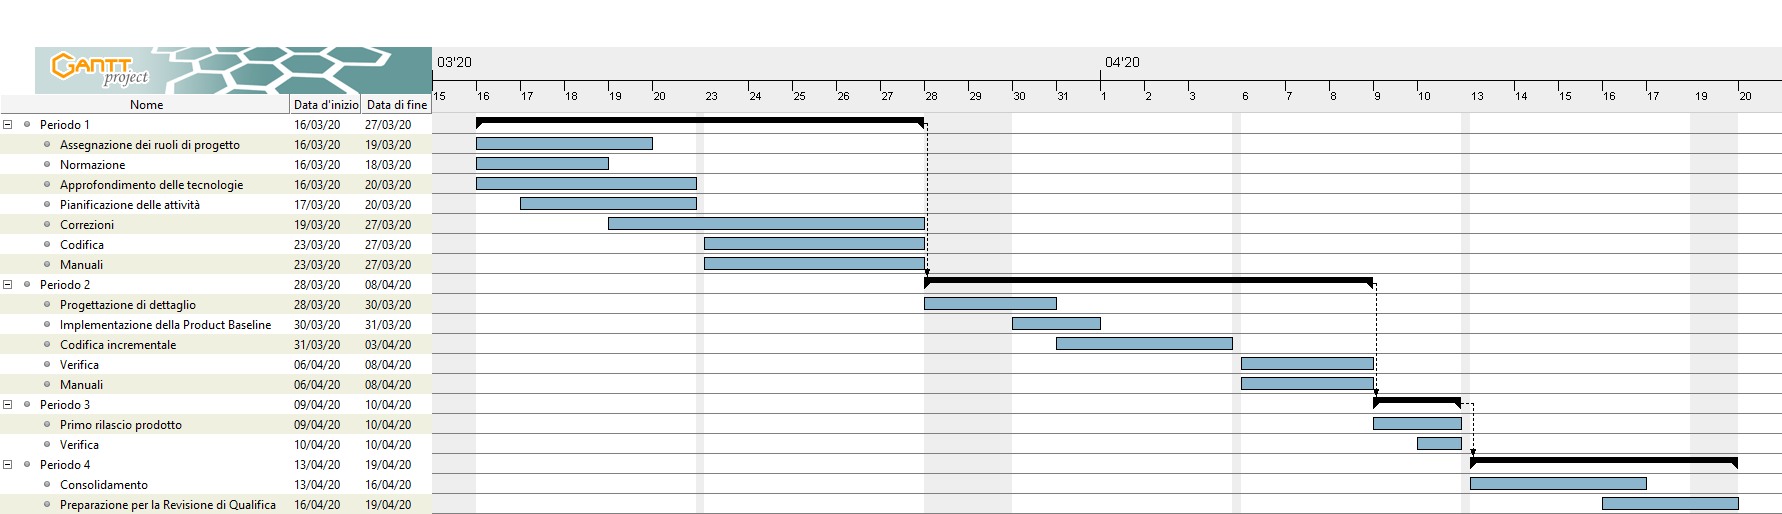
\includegraphics[scale=0.35]{Sezioni/DiagrammiGantt/ProgettazioneDiDettaglio.png}
	\caption{Diagramma di Gantt delle attività di Progettazione di Dettaglio e Codifica}
\end{figure}

\hrule
\vskip 6pt
Piano di Progetto \hskip 25cm {30} \rightline{30}
\end{landscape}
\clearpage